\chapter{Materiais e Métodos}
\label{chap:mat}
asdfasdfsdf

%--------- NEW SECTION ----------------------
\section{Especificação dos componentes}
\label{sec:espc}
asjdflkdjsaf

\subsection{Estrutura analítica do protótipo}
\label{ssec:pbs}
asdkjfsdalkjf

\subsection{Lista de componentes}
\label{ssec:list}
asfkjdsahfkjs


%--------- NEW SECTION ----------------------
\section{Diagramas mecânicos}
\label{sec:diagm}
asdfsdaf

%--------- NEW SECTION ----------------------
\section{Modelo esquemático de alimentação e comunicação}
\label{sec:modesq}
asdfadsfsdfs

\subsection{Diagramas elétricos}
\label{sec:diage}
asdfsdaf

\subsection{Esquemas eletrônicos}
\label{ssec:esqe}
asdfsdaf

%--------- NEW SECTION ----------------------
\section{Especificação das funcionalidades}
\label{sec:espf}
asdfadsfsdfs

\subsection{Fluxo das informações}
\label{ssec:fluxo}
asdfsaf

\subsection{Motion Planning}
\label{ssec:motion}
\subsubsection{Definição da funcionalidade}
A funcionalidade de \textit{Motion Planning} é responsável por realizar o planejamento da trajetória do Robô, utilizando o software \textit{MoveIt!} que realiza o cálculo da cinemática inversa para encontrar a melhor forma de ultrapassar os obstáculos.
\subsubsection{Dependências}
O software moveit pode utilizar o modelo matemático da cinemática inversa do robô ou um arquivo do tipo URDF.
O nome URDF é uma sigla para \textit{Unified Robot Description Format}, esse arquivo é uma especificação em \verb|XML| utilizada para descrever robôs. Modelos em URDF apresentam uma simplicidade na descrição do robô, e para o caso do Robô \textit{Elir}, utilizar o modelo URDF possibilitará uma aproximação fiel ao modelo real do robô, assim para o cálculo da cinemática inversa será utilizado o seu modelo URDF e não o seu modelo matemático.

\subsubsection{Premissas Necessárias}
Para o correto funcionamento dessa funcionalidade as seguintes premissas são necessárias:
\begin{itemize}
	\item A configuração dos limites de giro das juntas do robô estarão compatíveis com os comandos enviados
	\item O modelo URDF do robô estará adequado com o modelo físico
	\item O pacote gerado pelo \textit{MoveIt! Setup Assistant} estará configurado adequadamente
\end{itemize}
\subsubsection{Descrição da Funcionalidade}
A movimentação do robô na linha acontecerá por movimentos de translação e transposição de obstáculos. A translação na linha será feita por controladores de torque nas rodas do robô, enquanto a transposição do obstáculos utilizará o moveit.
Por meio da ferramenta \textit{MoveIt! Setup Assistant}, se utiliza o modelo do robô para criar um pacote do ROS com os principais arquivos pelo moveit. 
A configuração correta do moveit possibilita que se utilizem as funções da sua biblioteca para o cálculo da trajetória, levando em consideração também obstáculos no caminho.

O moveit fornece uma \textit{user interface} que recebe o end-effector,a nomenclatura atribuída ao node feito em python que recebe o \textit{end-effector} é \verb|moveit_commander|. O  \textit{node} responsável por fazer a integração da user interface com os parâmetros recebidos pelo \textit{ROS Parameter Server} com o \textit{end-effector} para fazer os cálculos é denominado \verb|move_group|. O \textit{node} \verb|move_group| também pode receber parâmetros como leituras dos sensores do robô e nuvens de pontos.

\begin{figure}[H]
	\centering
	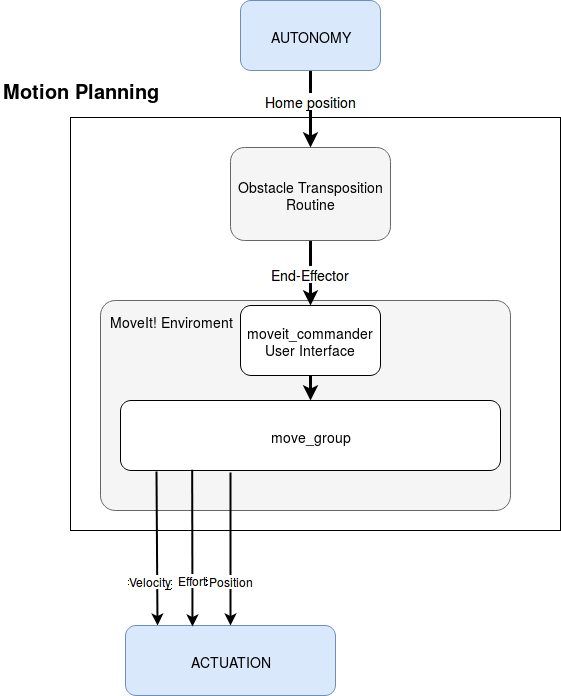
\includegraphics[width=0.8\textwidth]{motion_plan_func.png}
	\caption{Fluxograma de funcionamento da funcionalidade de Motion Planning}
	\label{fig:flux_motion}
	\source{Própria}
\end{figure}

\subsubsection{Saídas}
Por meio da compatibilização do \textit{MoveIt!} com o \textit{ROS}, a saída dessa funcionalidade são os comandos de velocidade, esforço e posição para cada junta do robô.

\subsection{Actuation }
\label{ssec:actu}
\subsubsection{Definição da funcionalidade}
A funcionalidade de Actuation tem como objetivo mover a estrutura física do robô, possibilitando o controle dos movimentos das juntas, garras e unidades de tração.
\subsubsection{Dependências}
Essa funcionalidade depende das funcionalidades de \textit{Power Management} e \textit{Motion Planning}. O \textit{Power Management} será responsável por fazer alimentação dos motores, possibilitando controlar a corrente máxima fornecida para cada grupo.
A dependência em relação à funcionalidade de \textit{Motion Planning} está atrelada principalmente com o software \textit{MoveIt!}, que ao receber um \textit{end-effector},realiza o cálculo de trajetória e envia os comandos de velocidade, esforço e posição para os controladores das juntas, garras e unidades de tração.

\subsubsection{Premissas Necessárias}
Para o correto funcionamento desse módulo, devem ser consideradas as seguintes premissas:
\begin{itemize}
	\item Os motores devem estar configurados de acordo com o padrão de ID determinado pela equipe, fazendo parte da mesma malha de controle;
	\item Os controladores das juntas,garras e unidades devem estar configurados de acordo com os comandos que serão recebidos pelo MoveIt!;
	\item Os 3 grupos de motores estarão em malhas de alimentação de 12V individuais.
\end{itemize}
\subsubsection{Descrição da Funcionalidade}
O ROS disponibiliza uma série de drivers para compatibilização dos motores dynamixel, possibilitando a criação de controladores específicos no seu ambiente. Serão criados os controladores referentes as juntas e unidades de tração do robô.Os controladores receberão comandos de \textit{velocity} e \textit{position} do \textit{MoveIt!} junto com os comandos para movimentar o robô na linha.
Após os comandos serem recebidos pelos controladores, eles serão enviados para o \textit{hardware} do robô, de acordo do padrão de comunicação dos motores, por meio de comunicação serial. 
\begin{figure}[h]
	\centering
	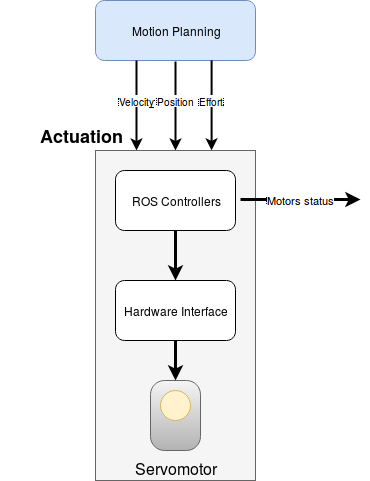
\includegraphics[width=0.6\textwidth]{actuation_depen.png}
	\caption{Fluxograma da funcionalidade Actuation}
	\label{fig:depen_actuation}
	\source{Própria}
\end{figure}
\subsubsection{Saídas}
A saída desta funcionalidade é o movimento da estrutura física do robô, que estará de acordo com o planejamento de trajetória do \textit{MoveIt!} e com as instruções para operação na linha

\subsection{Power Management}
\label{ssec:power}
\subsubsection{Definição da funcionalidade}

A funcionalidade de \textit{Power Management} é responsável por administrar o fornecimento de energia para os dispositivos eletrônicos do robô, nos níveis adequados de tensão e corrente.

\subsubsection{Dependências}
Essa funcionalidade depende da comunicação serial por meio da biblioteca \textit{rosserial} e da operacionalização do firmware embarcado no hardware (placa) de acordo com as necessidades do projeto.

\subsubsection{Premissas Necessárias}
Para o correto funcionamento desse módulo de \textit{Power Management}, devem ser consideradas as seguintes premissas:
\begin{itemize}
	\item A placa multiplexadora estará conectada diretamente ao módulo de \textit{Power Management} 
	\item Todos os dispositivos estarão conectados nas suas respectivas entradas
	\item A placa deverá ser alimentada por 2 baterias
	\item A placa estará conectada diretamente na NUC, por meio de uma USB	
\end{itemize}
\begin{figure}[h]
	\centering
	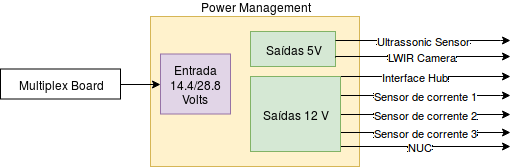
\includegraphics[width=1\textwidth]{power_management_hardware.png}
	\caption{Fluxograma de funcionamento da funcionalidade de Power Management}
	\label{fig:power_management_hardware}
	\source{Própria}
\end{figure}
\subsubsection{Descrição da Funcionalidade}
A placa de \textit{Power Management} fornece diversos recursos para integração com o ROS. Seu firmware, além de realizar as medições e controle dos níveis de tensão e corrente para alimentação do robô, estará adaptado com as seguintes funcionalidades para que haja integração do hardware com o ROS:
\begin{itemize}
	\item \textit{Publishers} que contém os status das portas em níveis de tensão e corrente; avisos de surtos de corrente ou sobre-corrente; disponibilidade do hardware de \textit{Power Management}
	\item \textit{Serviços} para realizar a verificação dos níveis de corrente; definição dos limites de corrente nas portas; realização de comandos on-off
\end{itemize}
O conjunto de baterias fornecerá a energia para o sistema, a placa de \textit{Power Management} irá administrar a distribuição da energia para os seguintes componentes:
\begin{itemize}
	\item Grupos de servo motores
	\item Grupo de sensores de corrente
	\item NUC
	\item Interface HUB
	\item Câmera LWIR
	\item Sensor ultrassônico
\end{itemize}

\subsubsection{Saídas}
A funcionalidade irá disponibilizar a energia para o robô e as seguintes estruturas no ambiente ROS:
\begin{itemize}
	\item Tópicos com informações de tensão e corrente nas portas
	\item Tópico para aviso de sobre-corrente
	\item Tópico para informar disponibilidade da placa
	\item Serviços para ler e configurar limite de corrente das portas
	\item Serviço para ligar ou desligar energia em uma porta	
\end{itemize}

\subsection{System Integrity Check}
\label{ssec:check}

\subsubsection{Definição da funcionalidade}
É a funcionalidade responsável por checar a integridade do sistema antes do início da missão, verificando os subsistemas e suas variáveis.

\subsubsection{Dependências}
A funcionalidade receberá informações dos seguintes componentes
\begin{itemize}
	\item Sensor de Temperatura
	\item Servomotores
	\item Câmera IR
	\item Câmera Stéreo
	\item IMU
	\item Sensor de Proximidade
	\item Placa de Power Management
	\item Sonar 
	\item Baterias
\end{itemize}

Todas as informações serão enviadas por meio do ambiente ROS, na forma de \textit{Services} ou \textit{Publishers}.

\subsubsection{Premissas Necessárias}
As premissas necessárias para o funcionamento dessa funcionalidade são:
\begin{itemize}
	\item Os subsistemas do robô irão disponibilizar o seu status no ambiente ROS por meio de tópicos ou serviços
	\item A checagem fará parte do planejamento de missão
\end{itemize}

\subsubsection{Descrição da Funcionalidade}
A checagem da integridade do sistema é uma funcionalidade essencial para garantir o sucesso da missão e preservar a integridade do robô. O ROS facilita essa comunicação entre os subsistemas, possibilitando que seja criada uma rotina de checagem antes de cada missão.

Será disponibilizado no sistema uma rotina para iniciar a missão. Ao receber o comando para início de missão, os sistemas serão checados sequencialmente, utilizando estrutura de \textit{Services} e \textit{Publishers} do ROS. Caso algum sistema apresente falha, a missão não se iniciará e o erro será mostrado no \textit{terminal} e registrado no arquivo de \verb|log|. Se todos os sistemas estiverem em funcionamento, se iniciará a missão. O fluxograma da funcionalidade está ilustrado na figura \ref{fig:sys_check_flux}.	
\begin{figure}[h]
	\centering
	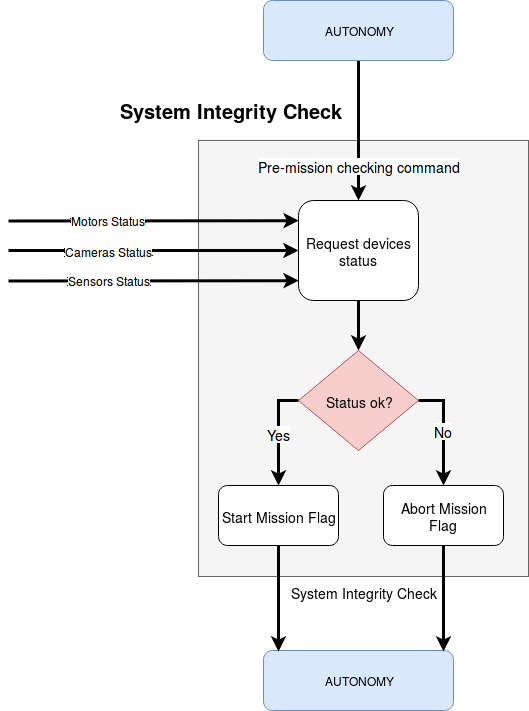
\includegraphics[width=0.6\textwidth]{sys_check_flux.png}
	\caption{Fluxograma da rotina para checagem do sistema}
	\label{fig:sys_check_flux}
	\source{Própria}
\end{figure} 


\subsubsection{Saídas}
No início da rotina de inspeção, a funcionalidade será responsável por enviar o sinal inicia a missão. Caso todos os sistemas checados estejam funcionando, a inspeção ocorrerá normalmente, se algum sistema apresentar defeitos, o defeito será mostrado no \textit{terminal}, registrado em log e a missão será abortada.
%--------- NEW SECTION ----------------------
\section{Interface do Usuário}
\label{sec:ui}
asdfadsfsdfs

%--------- NEW SECTION ----------------------
\section{Simulação do sistema}
\label{sec:sim}
asdfadsfsdfs


